\section{Results}

DETER data show an abrupt fall in during PRODES year 2019 followed by an increasing trend in the area covered by its alerts. It is worth noticing that the distribution by area in homogenous for each year, particularly for 2021 (see ~Figure~\ref{fig:deter_warnings_area_size}).

\begin{figure}[h] 
    \begin{center}
    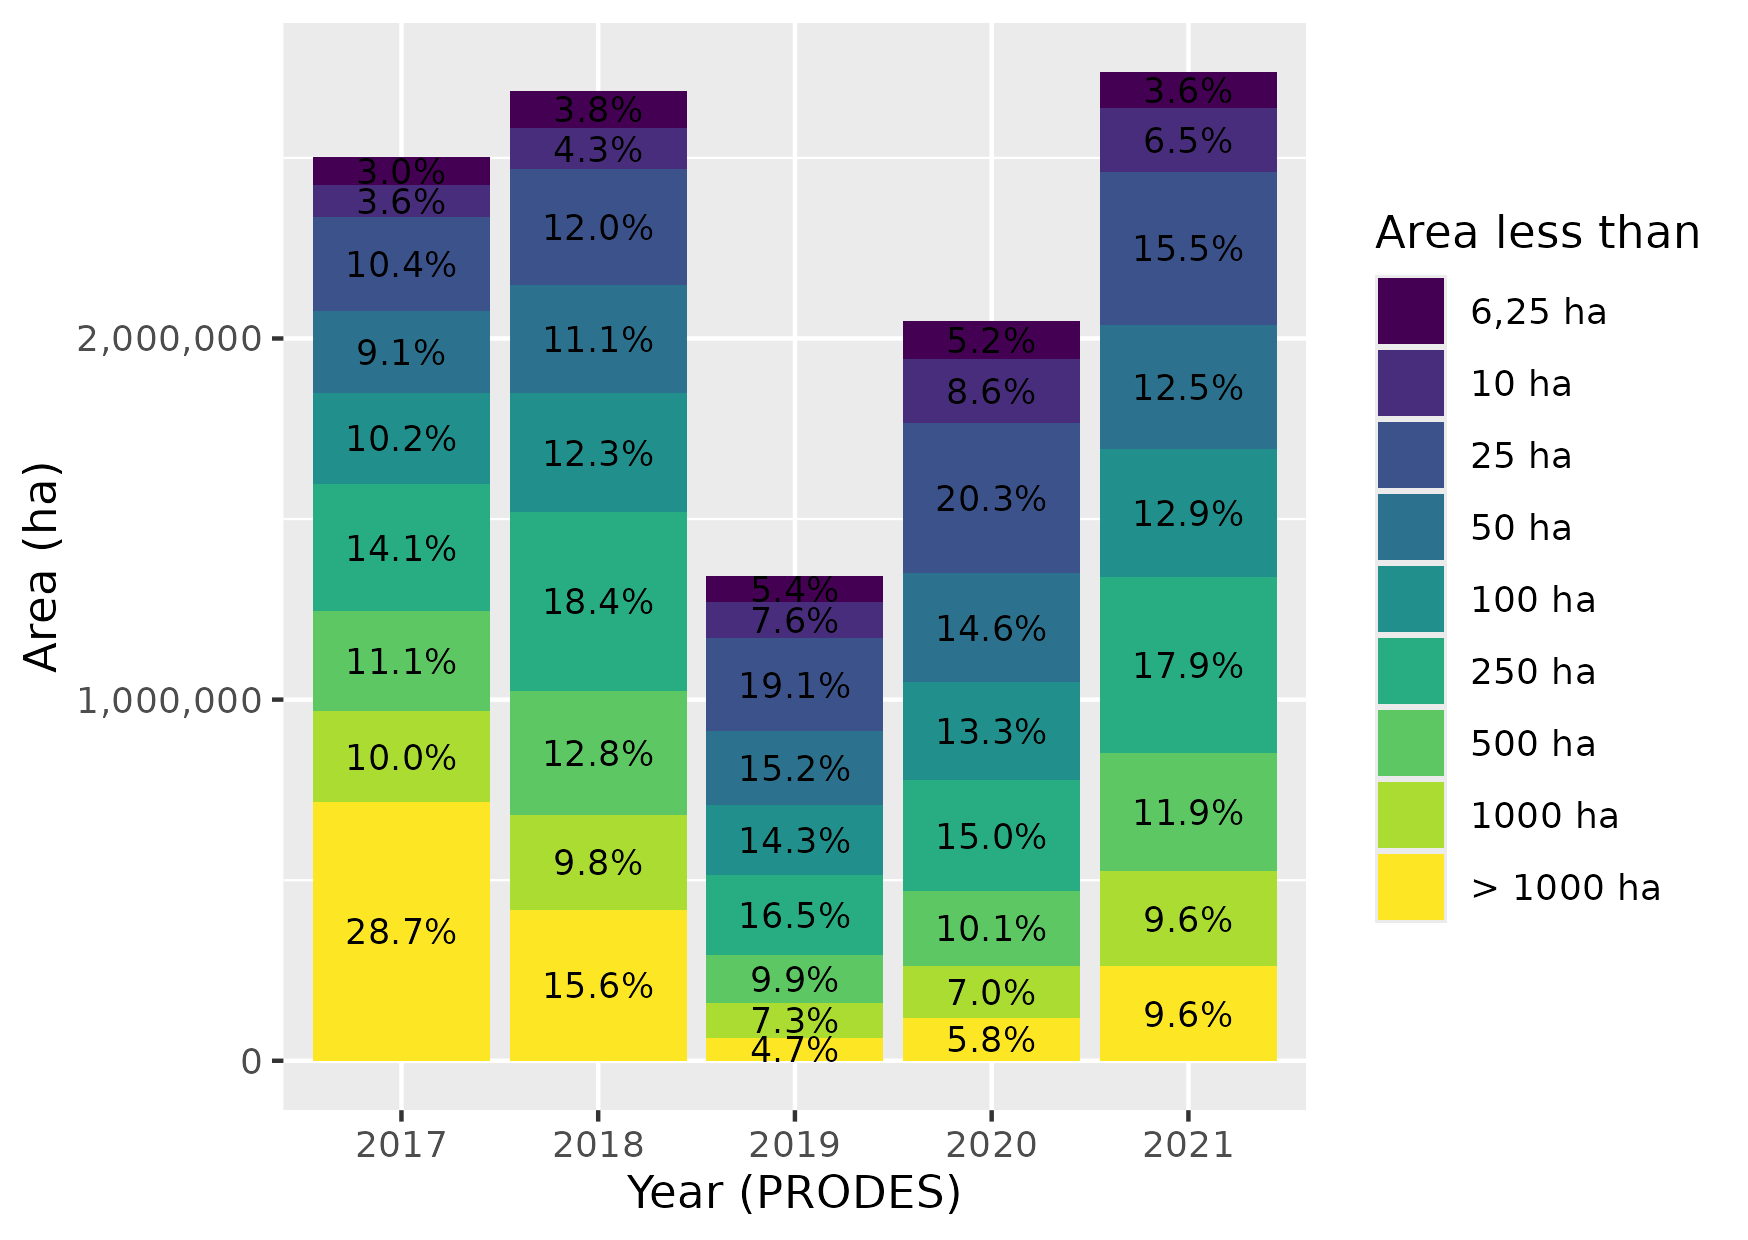
\includegraphics[width=\linewidth]{deter_warnings_area_size.png}
    \caption{Area of DETER alerts by year and size. The area covered by alerts
        peaked in 2018 and 2021. Note the increasing trend since 2019 and how
        their area distribution is relatively homogeneous along in 2021.}
    \label{fig:deter_warnings_area_size}
    \end{center}
\end{figure}

Moreover, the number of DETER alerts during the same period shows a somewhat similar pattern, characterized by the fact that half of yearly DETER alerts are issued for small areas (Figure~\ref{fig:deter_warnings_size}).

\begin{figure}[h] 
    \begin{center}
    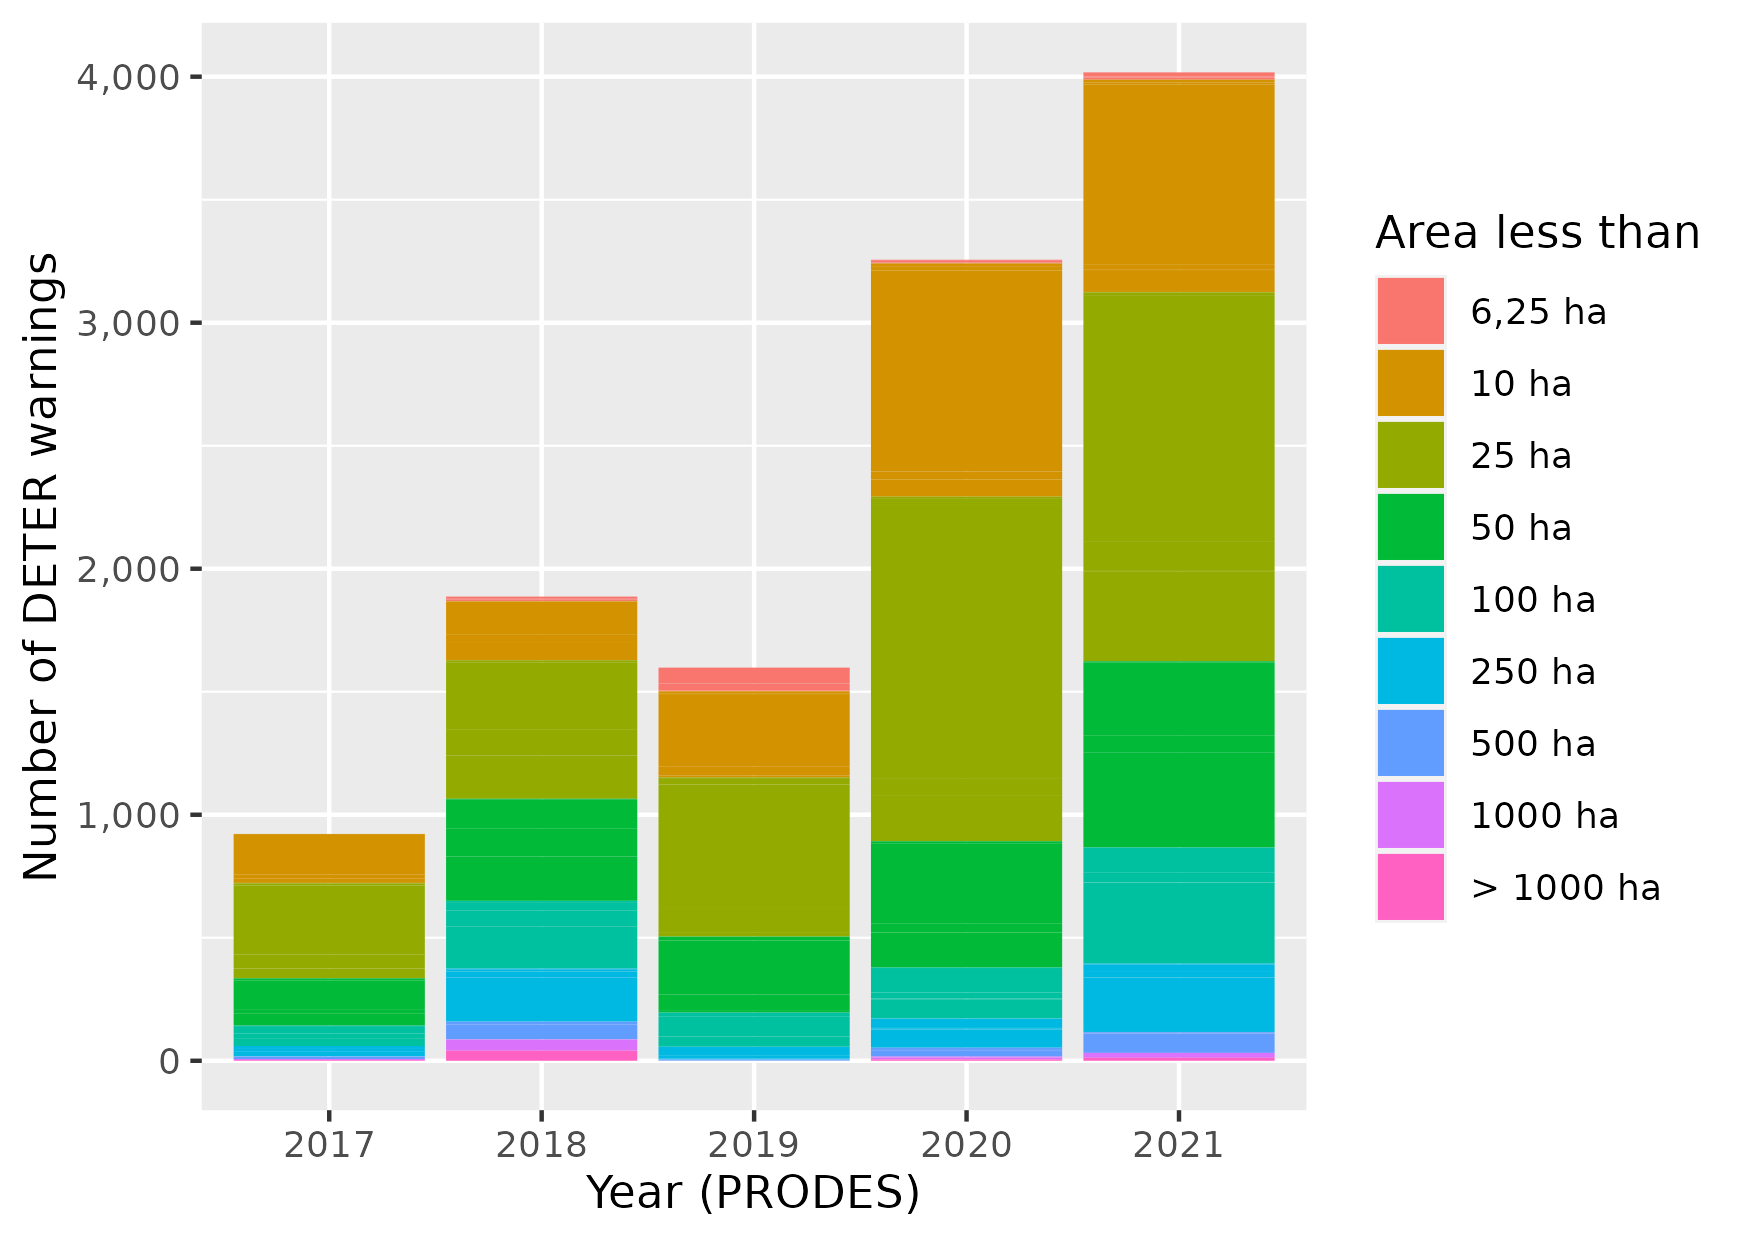
\includegraphics[width=\linewidth]{deter_warnings_size.png}
    \caption{Number of DETER alerts by year and size. Note the increasing trend
        since 2017. Note how DETER issued a similar number of alert in 2020 and
        2021 but ~Figure~\ref{fig:deter_warnings_size} shows a larger extent of
        alerts in 2021.}
    \label{fig:deter_warnings_size}
    \end{center}
\end{figure}

From August to October is when most DETER alerts are issued, and September, the peak month, presents an increasing trend in area, reaching its maximum in 2021.
This period corresponds to the fire season in most of the Brazilian Amazon~\cite{carvalho2021} (see Figure~\ref{fig:deter_warnings_size_month}). 

\begin{figure}[h] 
    \begin{center}
    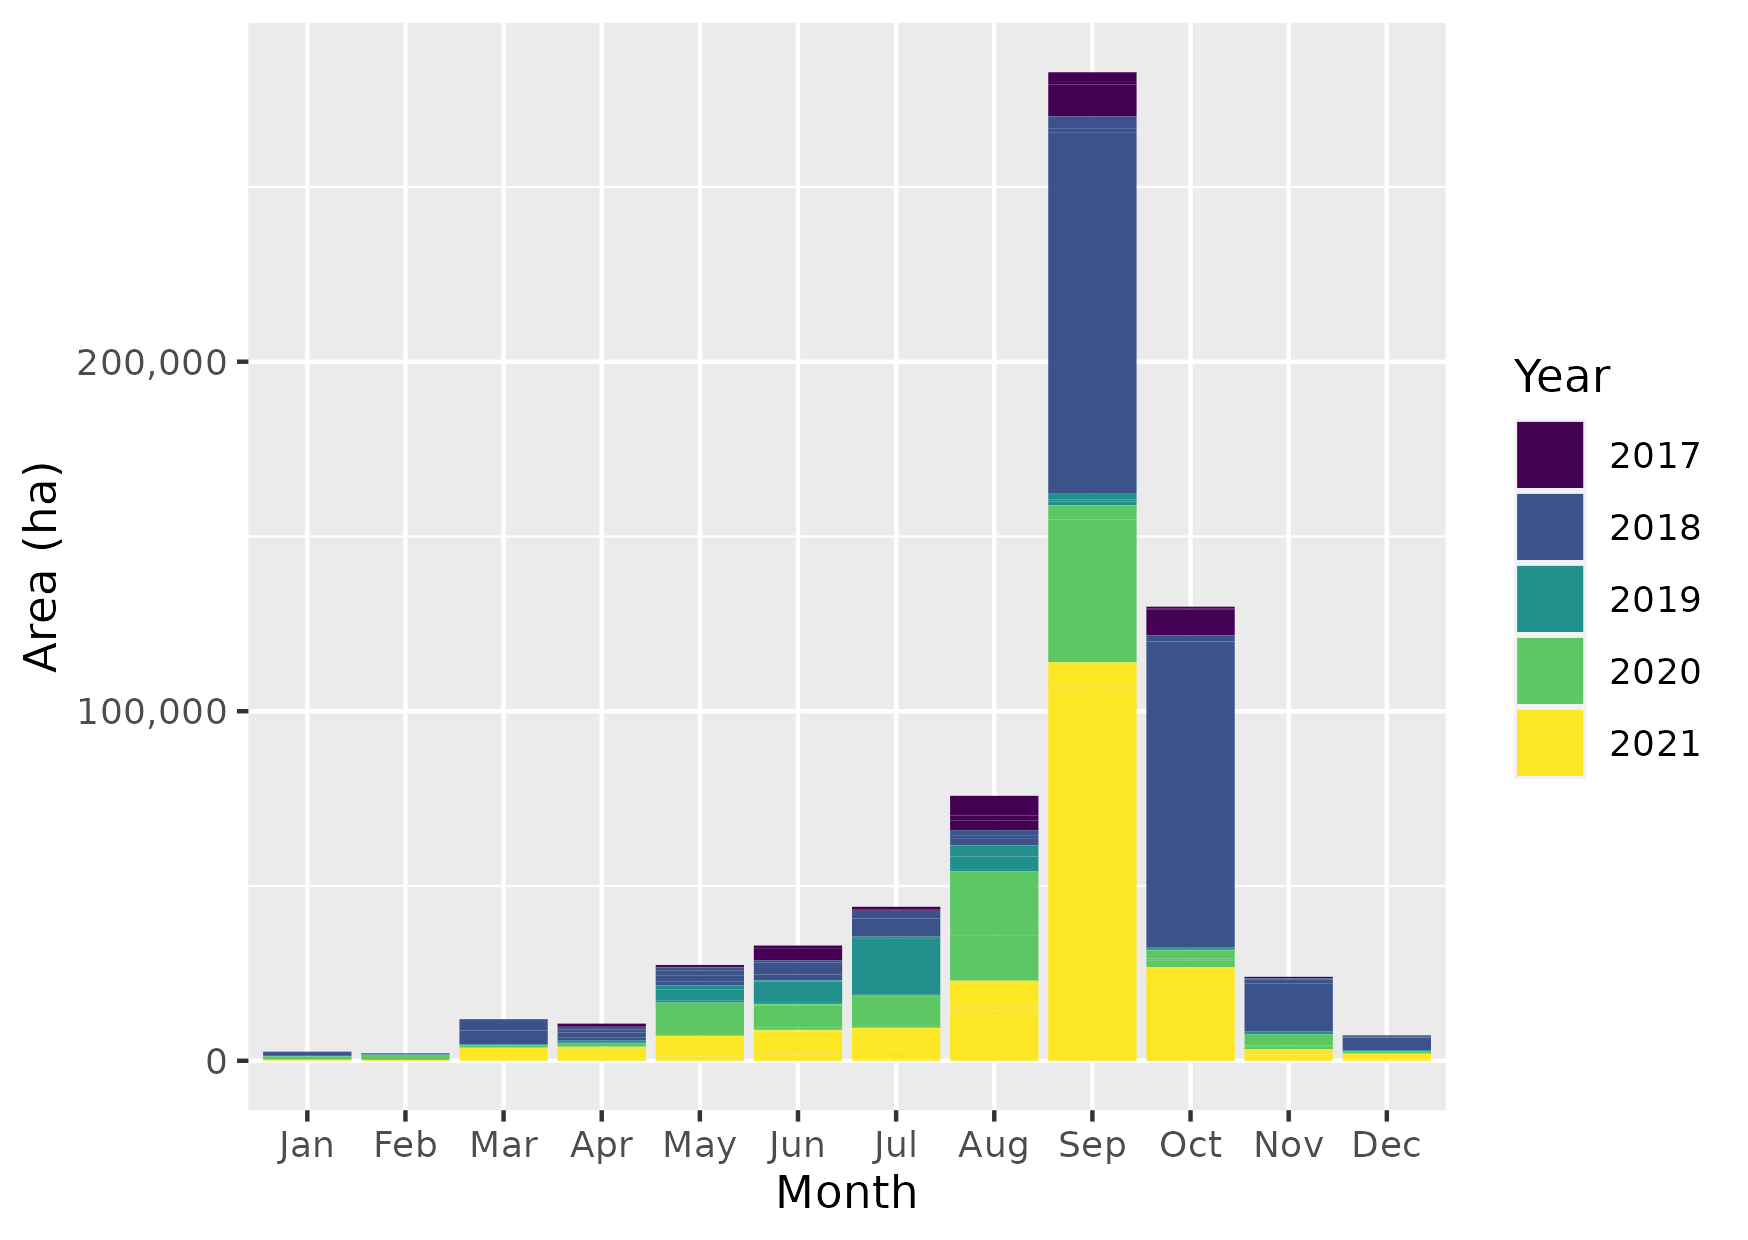
\includegraphics[width=\linewidth]{deter_warnings_size_month.png}
    \caption{DETER warnings by month. Between August and October is when most
        of the warnings are issued. Note how September presents an increasing 
        trend along the years which peaks in 2021.}
    \label{fig:deter_warnings_size_month}
    \end{center}
\end{figure}

Most DETER subareas are issued a single alert and never more than five, following an exponential decay pattern.

\begin{figure}[h] 
    \begin{center}
    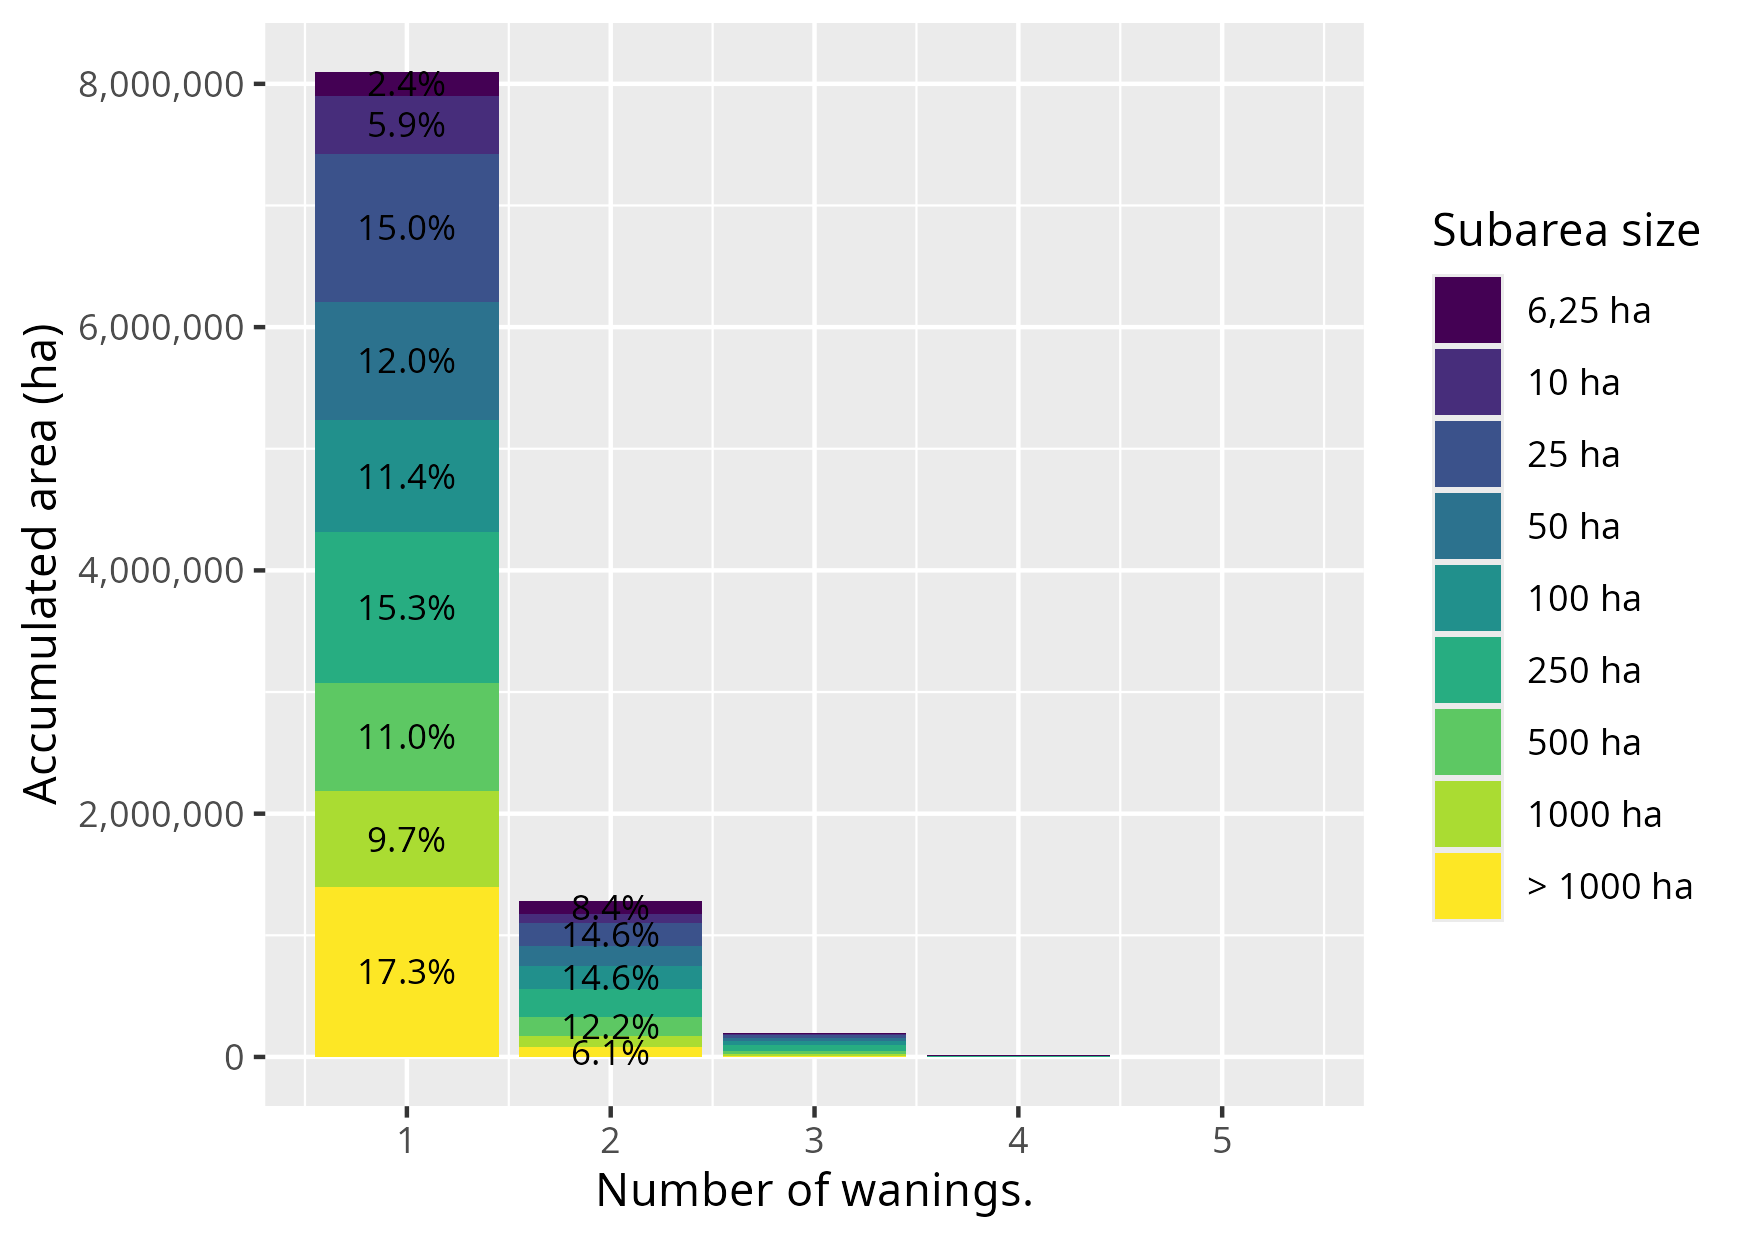
\includegraphics[width=\linewidth]{plot_area_by_warnings.png}
    \caption{DETER subareas by number of warnings. Most subareas only have one
        DETER alert and never more than five. The total extent for each number
        of alerts is homogeneously distributed.}
    \label{fig:plot_area_by_warnings}
    \end{center}
\end{figure}

%n_warnings,area_type,n_subareas,total_area_ha
1,"6,25 ha",749,3468.9305817097575
1,10 ha,2535,20277.63376261522
1,25 ha,4002,63098.2149548817
1,50 ha,1682,58496.47115551768
1,100 ha,847,58490.38486713717
1,250 ha,459,69741.03013061572
1,500 ha,133,43890.28044541861
1,1000 ha,54,36388.05024453305
1,> 1000 ha,42,108701.00171141527
2,"6,25 ha",617,2754.463872088673
2,10 ha,542,4300.325377400743
2,25 ha,829,13016.655436123781
2,50 ha,356,12588.702356866337
2,100 ha,200,14101.669591812615
2,250 ha,111,16949.55559907801
2,500 ha,25,8804.534433634506
2,1000 ha,12,8361.25238844781
2,> 1000 ha,3,6444.004258638234
3,"6,25 ha",70,331.8730328444766
3,10 ha,48,383.2278256572545
3,25 ha,62,943.440952612507
3,50 ha,15,528.551615276519
3,100 ha,5,342.0266654521489
3,250 ha,2,261.59856489548065
4,"6,25 ha",5,24.44017934602583
4,10 ha,1,8.426126639709947
4,25 ha,2,31.449280712276668


The time period between DETER alerts in the same subarea is one year, except for subareas with two alerts, when it is two years (Figure~\ref{fig:plot_days_first_to_last}). 

\begin{figure}[h] 
    \begin{center}
        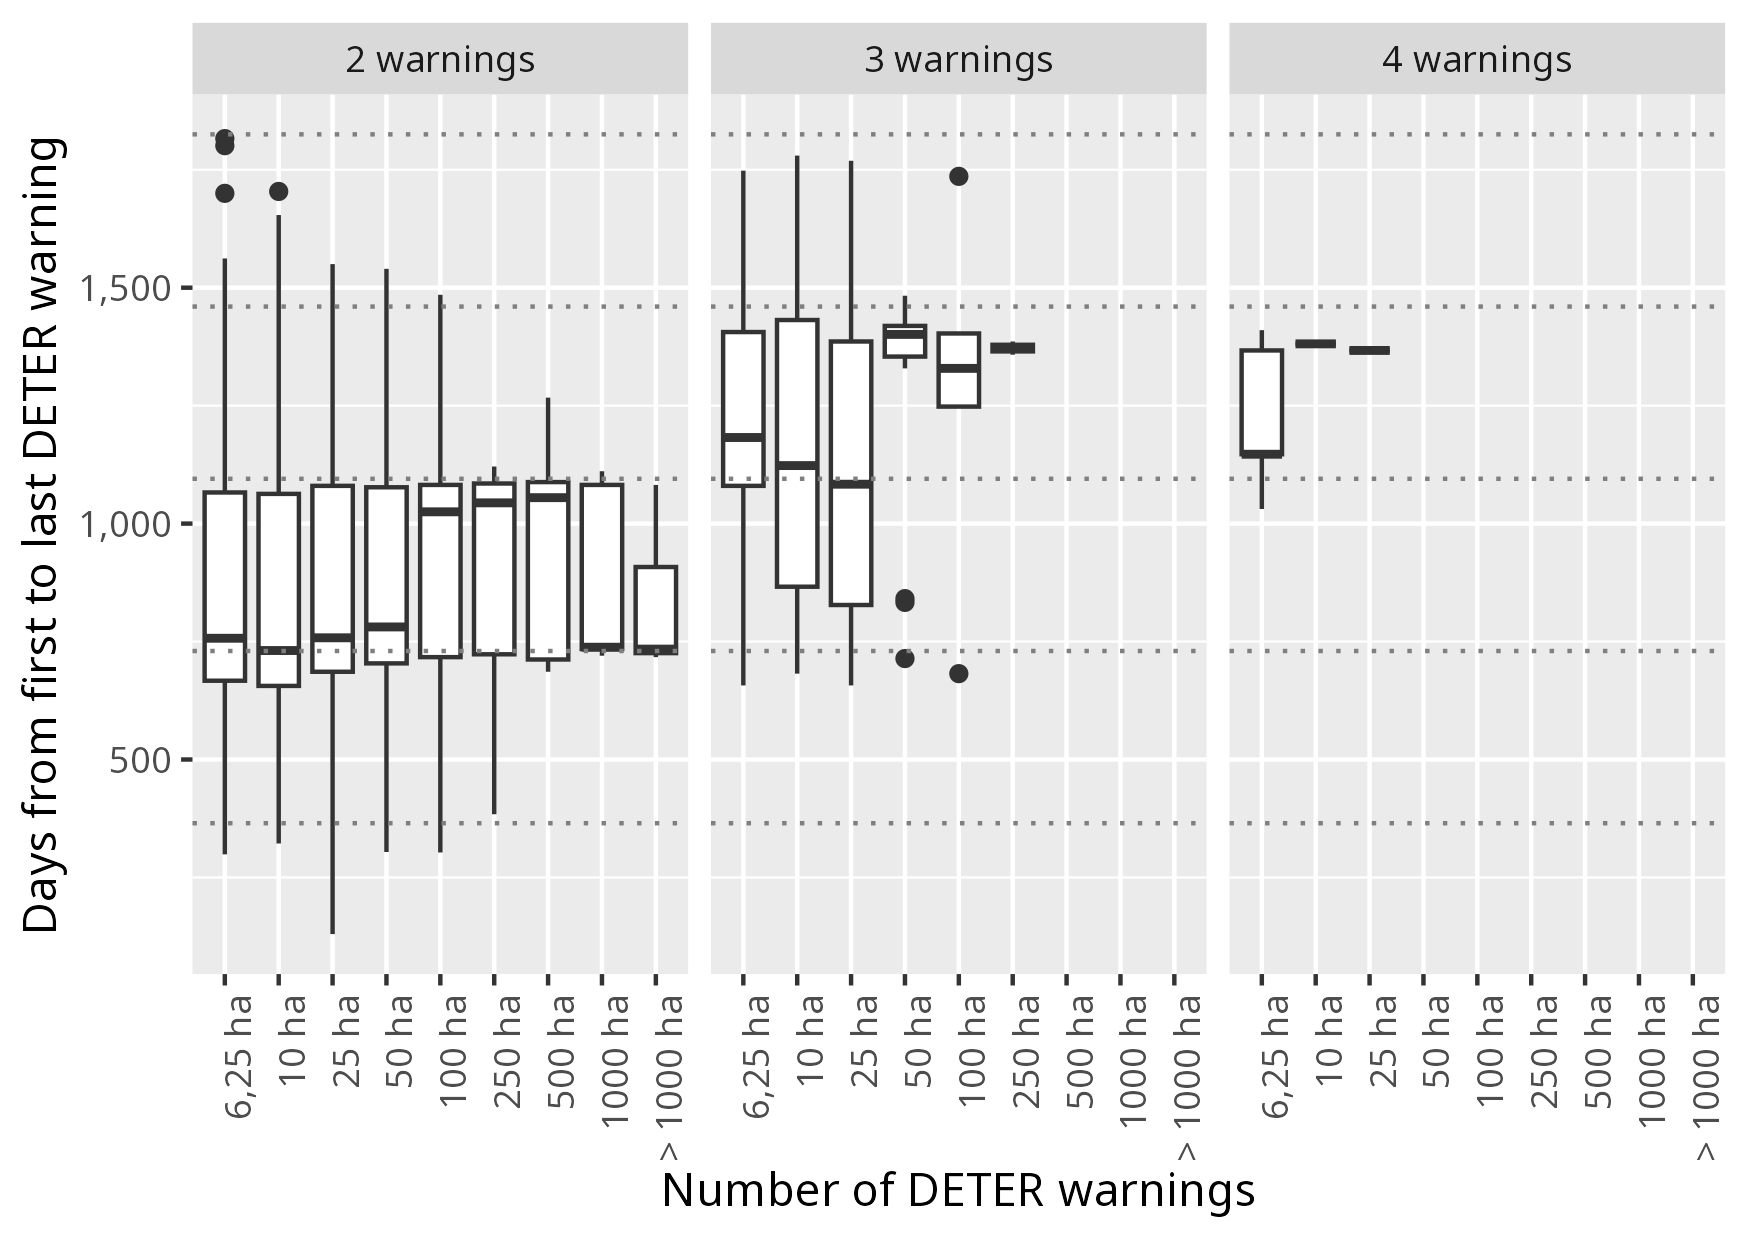
\includegraphics[width=\linewidth]{plot_days_first_to_last.png}
    \caption{Number of days between the first and last DETER alerts. The
        horizontal dashed black lines represent intervals of 365 days.
        DETER subareas with 2 warnings tend to be two years apart and then
        increase one year with each additional alert. Also note that the
        distribution by area tend to have long tails towards longer periods
        between the first and lat DETER alert.}
    \label{fig:plot_days_first_to_last}
    \end{center}
\end{figure}

The map in Figure~\ref{fig:plot_area_by_warnings} shows the distribution of recurrent deforestation warnings, that is, a surface interpolation of the number of DETER alerts.

\begin{figure}[h] 
    \begin{center}
        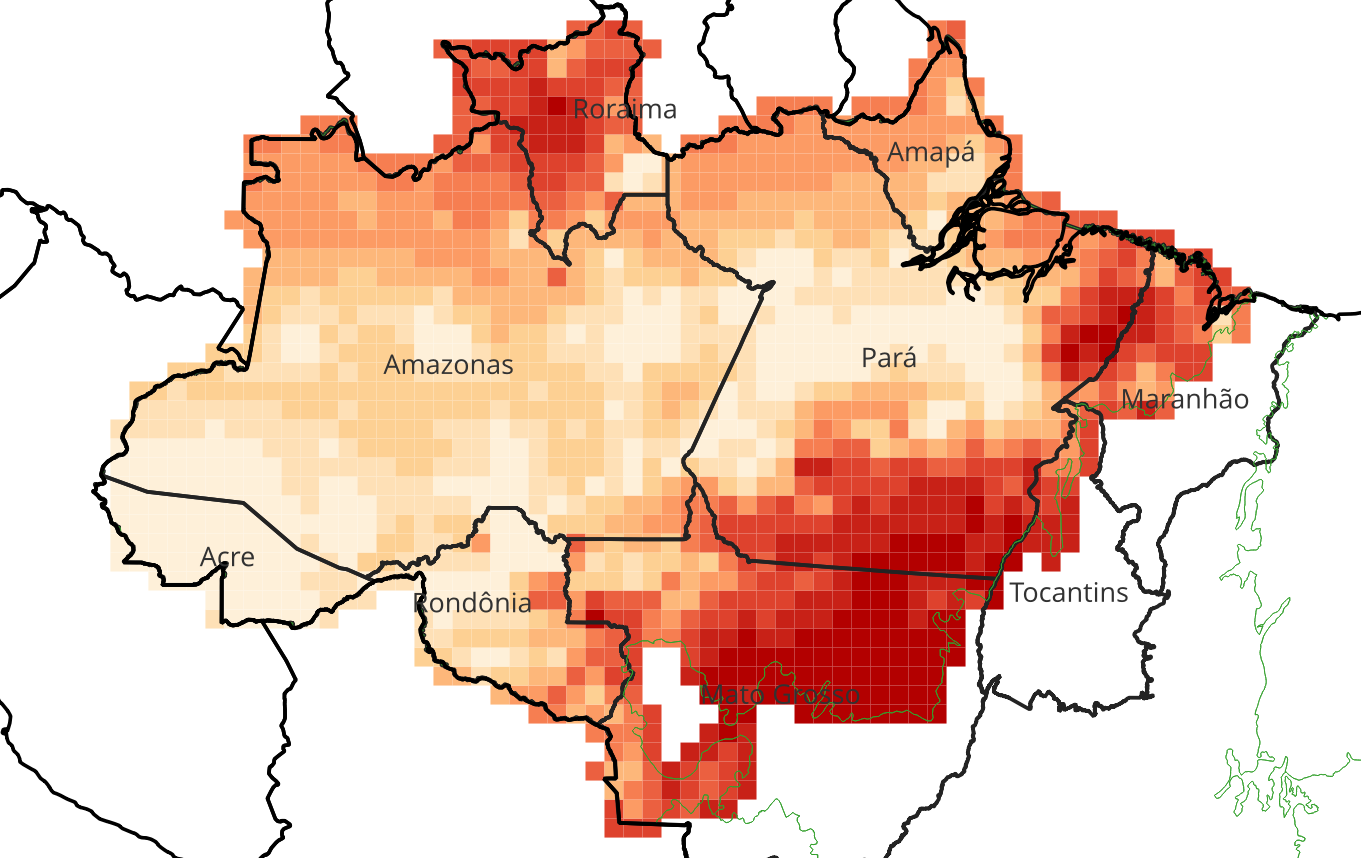
\includegraphics[width=\linewidth]{nwarnings_idw_map.png}
        \caption{Spatial distribution of recurrent degradation (number of
        alerts by subarea) in the Brazilian Amazon. Amazon's east front is
        where most of recurrent DETER alerts area found.}
    \label{fig:nwarnings_idw_map}
    \end{center}
\end{figure}
